\subsection{Søgemodul}
\label{sub:s_searchmodul}

Søgemodulet implementerer en sorteringsfunktion, som muliggør søgning på både og brugere.

\begin{figure}
  \centering
  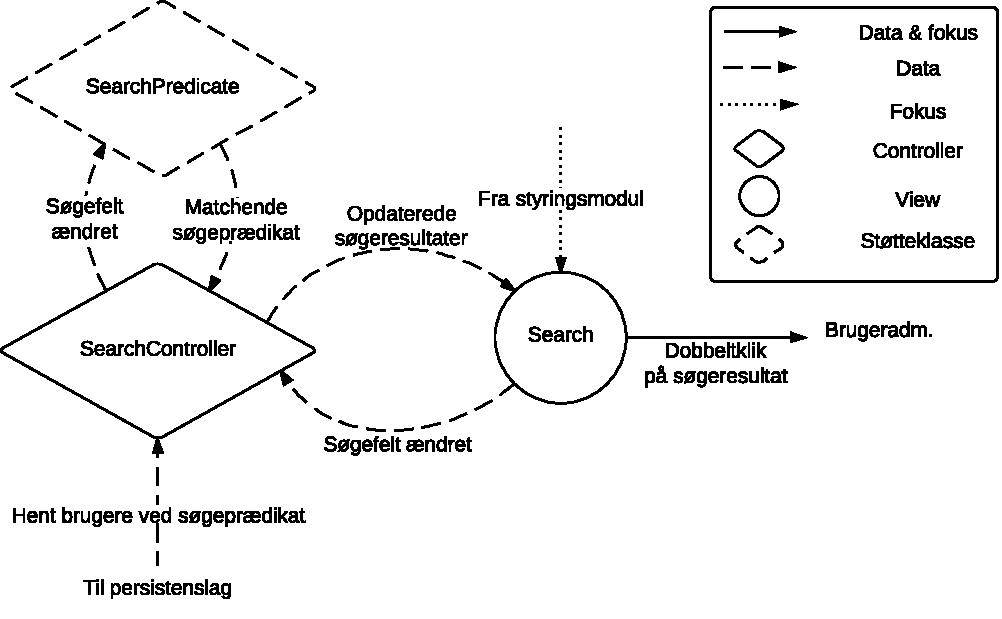
\includegraphics[width=\textwidth]{search-diagram.pdf}
  \caption{Dette er bare noget filler tekst.}
\end{figure}
\subsubsection{Funktionalitet}
\label{sub:funktionalitet}

Søgemodulets funktion er at sortere en liste af medlemmer og gæster, ud fra brugerdefinerede kriterier. Der kan sorteres efter alle datafelter som en bruger kan have. Derudover er det muligt at sortere efter datafelter som en brugers båd eller rejser indeholder.

\subsubsection{Implementation}
\label{sub:implementation}

Søgemodulet er inddelt i de følgende tre elementer:

\begin{itemize}
	\item \textbf{Søgebetingelseselementet} \\
		Dette element håndterer og validerer den information som en bruger måtte indputte. Ud fra disse oplysninger konstruerer betingelseselementet et unikt prædikat per datafelt. Dette prædikat tager en bruger som input, og returnerer en boolsk \enquote{sand}, hvis inputtet er en delstreng af brugernes pågældende felt.

	\item \textbf{Søgeelement} \\
    Søgeelementet har til formål at sortere en liste af bruger, på baggrund af prædikaterne fra betingelseselementet. Derudover står den også for at hente brugeroplysningerne fra databasen. Når søgeelementet bliver notificeret om, en ændring i en søgebetingelse, henter den det tilhørende prædikat fra betingelseselementet, og tilføjer prædikatet til en liste af søgekriterier. Ud fra denne liste sorteres listen af brugere, således at kun brugere, der returnerer \enquote{sand} for samtlige prædikater i listen af søgekriterier, bliver vist.

	\item \textbf{Bruger grænsefladen}
		Brugergrænsefladen har ansvaret for, at fremvise den sorterede liste, samt kalde sorteringsmetoden i søgeelementet når en bruger interagerer med brugergrænsefladen.
\end{itemize}

% subsection implementation (end)

% subsection funktionalitet (end)

% subsection s_gemodul (end)
